%\textit{A goal without a plan is just a wish} \\
%-- Antoine de Saint-Exup\'{e}ry 

% --------------------------------------------------------------------
% Preamble
% --------------------------------------------------------------------
\documentclass[a4paper]{article}	

\usepackage[scaled]{helvet}
\renewcommand\familydefault{\sfdefault} 
\usepackage[T1]{fontenc}

% 'microtype' can only be used with pdflatex
\usepackage[protrusion=true,expansion=true]{microtype}
	
\usepackage[utf8]{inputenc}
\usepackage[english]{babel}
\usepackage{amsmath}
\usepackage{stix}
\usepackage{bm}
\usepackage{graphicx}
\usepackage{xcolor}
\usepackage{enumitem} 	% Allows different styles in enumerate
\usepackage{ulem}		% For strikethrough text
\usepackage{rotating}	% For landscape figures

% Spacing between lines 
\usepackage{setspace}
\onehalfspacing

% ----- page layout 
\usepackage[
	a4paper,
	top=1in, bottom=1.25in, left=1.25in, right=1.25in
]{geometry}	

\setlength{\oddsidemargin}{5mm}			% Remove 'twosided' indentation
\setlength{\evensidemargin}{5mm}

% ----- To allow cross-referencing between documents
%       a common root folder must be established
%       this command encapsulates the path
\newcommand{\gsdPath}{../guidelines_software}%

% ------ To cross reference other documents
\usepackage{xr-hyper}
\usepackage[
	colorlinks=true,
	urlcolor=magenta,
	linkcolor=blue, 	% [red]
%	anchorcolor 	 % [black]
	citecolor=blue, 		% [green]
	filecolor=cyan, 	% [cyan]
	menucolor=black		% [red]
]{hyperref}

% Header and footer control
\usepackage{fancyhdr}
\setlength{\headheight}{15.2pt}
\pagestyle{fancy}

% ----- Table of contents 
\usepackage{titletoc}
\usepackage{tocloft}

\renewcommand\cftsecfont{\normalfont}
\renewcommand\cftsecpagefont{\normalfont}
\renewcommand{\cftsecleader}{\cftdotfill{\cftsecdotsep}}
\renewcommand\cftsecdotsep{\cftdot}
\renewcommand\cftsubsecdotsep{\cftdot}


% ----- Tables
\usepackage{booktabs}
\usepackage{colortbl}
\usepackage{longtable}
\usepackage{makecell}

% ----- Units formatting 
\usepackage{siunitx}

% ------ Macros for this document
\definecolor{yellowMSL}{RGB}{244,182,8}

% Mark-up for small changes (a few words only)
\newcommand{\proposed}[1]{{\color{cyan}{{#1}}}}
\newcommand{\deprecated}[1]{{\color{yellowMSL}{#1}}}

% Mark-up  for paragraphs. 
\usepackage{framed}
\newcommand{\proposedbox}[1]{
\colorlet{shadecolor}{gray!10}
{\color{cyan}\begin{shaded}
	{#1}
\end{shaded}}
}%

\newcommand{\deprecatedbox}[1]{
\colorlet{shadecolor}{gray!10}
{\color{yellowMSL}\begin{shaded}
	{#1}
\end{shaded}}
}%

% --------------------------------------------------------------------
% Front page definitions (do not change this)
% --------------------------------------------------------------------
\newcommand{\HRule}[1]{\rule{\linewidth}{#1}} 	% Horizontal rule

\makeatletter							% Title
\def\printtitle{%						
    {\centering \@title\par}}
\makeatother									

\makeatletter							% Author
\def\printauthor{%					
    {\raggedright \Large \@author}}				
\makeatother							


% --------------------------------------------------------------------
% Details of what to put on the front page (Change this)
% --------------------------------------------------------------------
\title{	\Large 
	\textsc{ Measurement Standards Laboratory of New Zealand } \\ [2.0cm]			
	\HRule{2pt} \\ [0.25cm]						
	\LARGE \textbf{\uppercase{Measurement Uncertainty Guidelines}}	\\% Title
    \Large \textit{A supplement to the MSL Quality Manual}
	\HRule{2pt} \\ [0.25cm]		
	\Large \today			
}

\author{
{\large 
	Text in this \proposed{colour} is awaiting approval by the 
	Quality Council.\\ 
	Text in this \deprecated{colour} is deprecated 
	and awaiting approval to be deleted.
} 
\\[\baselineskip] 		
Measurement Quality Council\\	
Measurement Standards Laboratory of New Zealand\\	
}


\begin{document}
\hypersetup{pageanchor=false}	% prevents a warning message
\fancyhf{}	% Header and footer are empty

% ------------------------------------------------------------------------------
% Title page
% ------------------------------------------------------------------------------
\thispagestyle{empty}		% Remove page numbering on this page
\pagestyle{plain}			% puts pages numbers back in front matter

\printtitle					% Print the title data as defined above
  	\vfill
\printauthor				% Print the author data as defined above
\newpage

\pagenumbering{roman}

\tableofcontents
\newpage

% ----- Main document now begins
\pagestyle{fancy}			% Turn on footer style control
\pagenumbering{arabic}
\hypersetup{pageanchor=true}
\setcounter{page}{1}		% Set page numbering to begin on this page

\fancyfoot[L]{Software}
\fancyfoot[C]{\today}
\fancyfoot[R]{Page \thepage\ of \pageref*{LastPage}}

\setlength{\parindent}{0cm}	% No indent when starting a new paragraph
\setlength{\parskip}{\baselineskip}	% Leave a blank line between paragraphs

% ----- These files contain the document content
\section{Introduction}
Every section in MSL relies on a suite of software tools for acquiring data, processing data and presenting data. No two sections use the same set of tools; most sections have developed bespoke solutions that suit their needs; there are a few cases of software being developed externally under contract.  

The quality system imposes a common set of requirements on the software used to carry out test and calibration work: it must be fit-for-purpose, it must demonstrably meet the design requirements of the task to be performed, and the integrity of software must be maintained. 

There is also a requirement to maintain the integrity of all measurement data. 

A few relatively simple practices can be followed to improve software quality and help meet the sorts of requirement faced by MSL. There are also useful software tools available. 

When writing new software in a modern programming language, these tools and practices can be incorporated without much effort. However, much of our software is in the form of `legacy' programs: software that may be modified from time to time, but which is unlikely to be redeveloped from scratch. 

Another difficulty is that some sections have invested heavily in types of software that are designed for programming by the end-user. This inherent flexibility makes them hard to maintain: spreadsheets being the best (or worst) example. Spreadsheets are convenient for quick work, but hard to validate and notorious for hiding errors.

Given the wide variety of software in use at MSL, the most useful guidance is likely to be a collection of simple ideas that can be adapted to a wide range of applications. The purpose of this document is to provide such general guidance.


\clearpage
\section{Style and Structure}
\begin{flushright}
\textit{“If you don’t know where you’re going, any road will take you there.”} \\
-- George Harrison 
\end{flushright}


Software should be developed with end-users and future owners in mind – it should also be designed to be tested and maintained easily. This requires consideration of how software is written.

\subsection{Style}
When writing, consideration should always be given to stylistic conventions: be consistent in your use of a simple, clear, style. A worthy goal is to write software that is \textit{self-explanatory}. This can be achieved by appropriate use of: names, data structures, programming structures and idioms, layout and comments. 

\paragraph{Names}
Careful naming is important. Names for variables, functions and classes, etc, should be
\begin{itemize}
\item easily remembered
\item concise
\item descriptive (for readers)
\item consistent (with names of similar entities)
\item easy to chose 
\end{itemize} 

Languages such as Visual BASIC, Python, C++, etc, and some end-user tools (e.g., MathCAD) allow considerable freedom to choose names. 

\paragraph{Data structures} All programming languages support a few basic data structures (e.g., arrays), some allow \textit{ad hoc} structures to be defined for particular uses (e.g., object-oriented structures). Good design of data structures is important, because it can make instructions that manipulate data easier to read, understand and maintain.

\paragraph{Programming structures and idioms} Authors in languages like English, etc, use syntactical rules and common idioms to write statements that can be easily understood. The same applies to programming. Each language has its own syntax, features and quirks, but there will always be good, widely-recognised, ways of describing common tasks, which can be regarded as `best-practice'.

All programming languages have a few basic control structures (e.g., \texttt{FOR-NEXT} loops, \texttt{IF-THEN} statements, etc). While the logic of these structures is simple and universal, the way they are deployed is usually language-dependent. There are subtleties in how the language works that make certain idioms preferable. Using recognised language idioms both improves code quality and makes it easier to read and maintain. 

  

\paragraph{Layout} The way that code appears on the page (screen) is important. Often source code will work fine no matter how it is laid out, but consistent layout makes a huge difference to readability. Once again, languages tend to have different conventions. Python even incorporates layout in the syntax of its block statements, in a deliberate effort to make code easier to read.

\paragraph{Comments} Software comments are something of a necessary evil: they should be used sparingly. It is better to revise code, considering appropriate naming, layout and idioms, because doing so may make a comment unnecessary.

While changes are made to code over time, comments are often overlooked. So, comments can drift with respect to the corresponding code base. Later, it may become unclear just how accurate a comment is. Writing code that does not need many comments is a better strategy. Only details that cannot be inferred from a clear coding style should be added as (preferably) short local comments.

\clearpage
\section{Data management}
\begin{flushright}
\textit{No problem is too small or too trivial if we can really do something about it.} \\
-- Richard Feynman 
\end{flushright}


Digital data and associated software are critical MSL assets. Like any other assets, they should be cared for and maintained. This section is about data management planning. 

\subsection{Data management planning}
MSL should identify its requirements for data management so that implementations (specific procedures as well as supporting IT services) can be evaluated. 

A Data Management Plan (DMP) describes how data is managed, from initial production, through data processing to, finally, long-term storage. It should cover how data is handled, who is responsible, and how adherence to the plan will be monitored.

The DMP should contain sufficient detail to enable stakeholders (MSL staff, managers, and IT support) to understand the requirements for data management.

\subsubsection{Points to be considered in a data management plan}
\begin{enumerate}
 \item How is data generated? What software is used? 
 \item Data formats (e.g., raw text, .csv, .xlsx, XML, etc). 
 
Open, non-proprietary formats are likely to remain usable longer. As a general rule, plain text formats, such as comma- or tab- delimited files, are open formats and are typically better for re-use and long-term preservation. Formats with complete and freely available documentation are more likely to remain usable. Avoid formats that can only be accessed by one program, e.g.: a Photoshop .psd file is proprietary whereas a .tiff image file is open.

Avoid formats that compress information in a file. They are often smaller, but the compression may permanently remove data. 

Avoid encrypted and compiled formats. Source code has a higher likelihood of remaining usable, since compiling is possible on different architectures and platforms.

 \item Is data annotated (with metadata)? Are standards used (which)? 
 \item Where is data stored? How is it organised (common file structure, database, etc)? 
 \item Size of data (storage and networking requirements)? 
 \item How is initial (raw) data secured? Level of protection required? 
 \item How is data processed? What software is used? 
 \item How is integrity maintained? Is there an audit trail?
 \item Do policies limit access to, and sharing of, (raw or processed) data? How are these policies implemented?
 \item How are final (published) reports and data related (records of processing, work flows, etc)?
 \item How is data, records of work flows, etc, archived? 
 \item How is software maintained (over time)?
 \item How long must data and software be retained?  
 \item Responsibilities for data (stewardship, custody)?\footnote{A `custodian`  is usually a manger with responsibility for the business function of data; they will have responsibility for planning and policy-making on data management. A `steward` is a subject-matter expert with responsibility for how data is used; they perform the work to manage data.}
 \item Who is responsible for the DMP (audits, reviews, etc)? Responsibility must transfer if key personnel leave. 
\end{enumerate}

\subsubsection{17025 requirements}

All commercial calibration data, unless explicitly noted otherwise, will be confidential to MSL (17025 clause 4.2).

When technical records are in the form of electronic data, they shall be maintained according to 17025 clauses 7.1.

Electronic data management systems used by MSL shall comply with clauses 7.11 of the standard, which deals with control of data and information management.

The control of all records shall comply with clauses 8.4 of the standard, which deal with the control of records.

\subsubsection{Example: A DMP for RF standards}
\paragraph{Raw data} is produced by bespoke data acquisition software written in Python. A github repository is used to store this data on the corporate file server, which is cloned on lab and office machines. 

\paragraph{Data acquisition} software is developed under version control using a cloud-based repository (github). A record of the version(s) used during a job is logged when raw data is collected.  

\paragraph{The data formats} used are mainly: plain text files, spreadsheet files (.xls and.xlsx) and Python source (text files with extension .py). The text and Python files are largely for storing configuration information and metadata; spreadsheet files contain measurement data. Results of data processing are also generated in plain text and in spreadsheet files; there is also one proprietary binary file format used for some data (the GTC archive). 

Note, there are no spreadsheet software requirements. Spreadsheets containing data may used for \textit{ad hoc} calculations but the main data analysis is done in Python. 

No metadata standards are followed. 

\paragraph{Data is organised} in a hierarchy of sub-folders under a job-specific root folder; sub-folder names are generally composed of a time-stamp added to a descriptive root (e.g., Fig.~\ref{fig:runs} shows sub-folders where the `sp' stands for S-parameters). The results of data processing are stored in a similar way, using folder names that begin
with `dp' followed by a date and time stamp (see Fig.~\ref{fig:folders}) 

The storage requirement for a completed job is typically several megabytes.

\begin{figure}[ht]
 \centering
  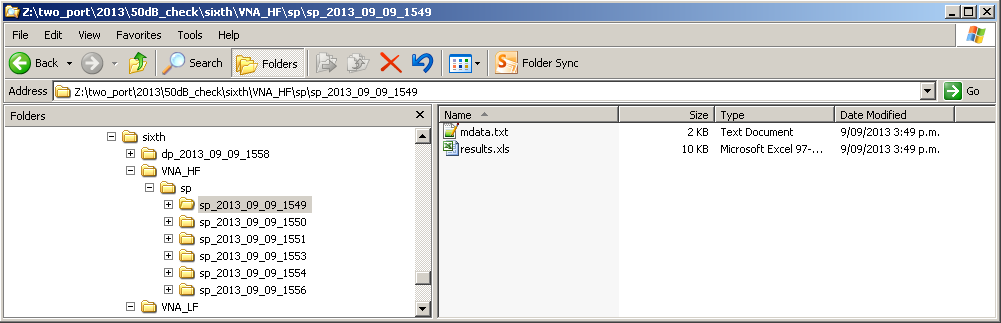
\includegraphics[width=0.8\linewidth]{pictures/filesystem_vna_runs.png}
  \caption{Measurement runs (sub-folders) inside an `sp' measurement folder (pane on the left) and the contents of one run folder (pane on the right).}
  \label{fig:runs}
\end{figure}

\begin{figure}[ht]
 \centering
  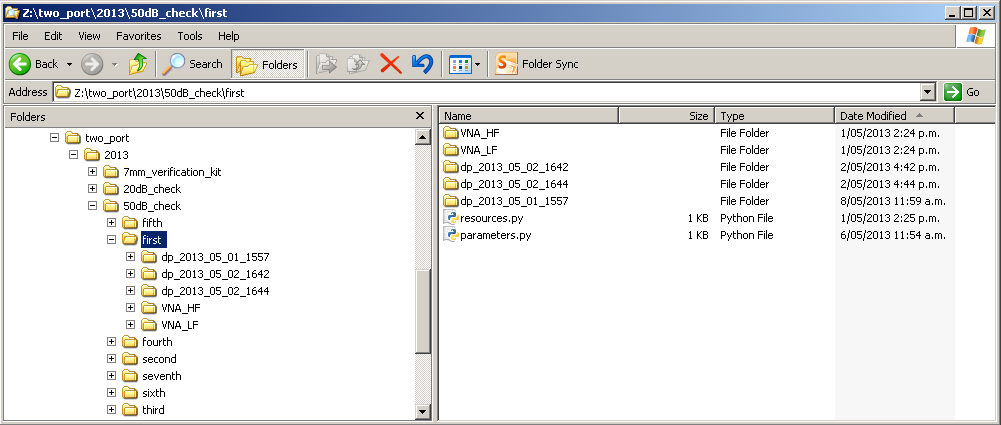
\includegraphics[width=0.8\linewidth]{pictures/filesystem_runs.png}
  \caption{View of a root folder structure for one job (the root is `first', organised below `two\_port', the year, and `50dB\_check'), containing three data processing sub-folders as well as VNA sub-folders in which raw data and configuration information is stored.}
  \label{fig:folders}
\end{figure}

\paragraph{Data integrity} is maintained by a git repository for each job. The initial job set-up creates a bare repository on the corporate file server (I-drive), which is immediately cloned to the lab computer. After raw data has been collected, it is committed to the local repository by the metrologist and a copy is pushed to the I-drive. 

This produces a (complete and independent) lab copy of the data and a remote copy on the I-drive; the I-drive is also routinely backed up by IT service (24-hour cycle). 

Using a repository guards against unintended accidental changes to data and also guards against intermittent network problems, by allowing work to be carried out locally until network access is restored.

\paragraph{All data} collected in commercial jobs is confidential to MSL by default. So, the `private' I-drive allocated to MSL is used, which restricts access to MSL staff. No other privacy protections are necessary.  

\paragraph{Data is processed} by bespoke Python software (also version-controlled) and the results stored in the same folder structure (see Fig.~\ref{fig:folders}). This allows the git repository to capture all stages of analysis. Using a git repository also facilitates review of processing details at a later date, or independent processing on the data without loss of information obtained earlier. 

When final client-specific analysis steps are required, the Python script for these last steps will be stored in the section file system commercial job file, which is separately located on the I-drive. The final report is also saved in this commercial job file. 

\paragraph{On completion} of a job, the repository is left undisturbed on local computers and on the corporate file server. There is no specific `archiving' process. The amount of data does not warrant compression and any eventual future analysis will be facilitated by maintaining the local file structure. 

Data and software must be retained indefinitely. 

The reliance on open-source Python software will help to provide on-going access to the functionality of our software. Python, of course, evolves and regular upgrades are expected. A suite of unit-test cases are used to facilitate migration and acceptance-testing of new versions.

\paragraph{Responsibilities} for data relate to custody and stewardship. The MSL Director is the nominally the custodian of data, but this is delegated to the Team Manager in charge of the section. The data stewards are MSL staff  qualified for the measurement procedure (MSL Competency Matrix). 

Adherence to the DMP will be reviewed annually and a record of review kept in the section files (lab book). 
\clearpage

\appendix	% Changes the style of the headings for sections
% \section{Abbreviations}
\begin{center}
{\renewcommand*{\arraystretch}{1.4}
\begin{tabular}{p{14.07em}p{25em}}
	\rowcolor[rgb]{ 0,  0,  0} 
	\textcolor[rgb]{ 1,  1,  1}{\textbf{Abbreviation}} & 
	\textcolor[rgb]{ 1,  1,  1}{\textbf{Stands For}} \\
APMP & Asia Pacific Metrology Programme \\ 
BIPM & Bureau International des Poids et Mesures \\ 
CC & Consultative Committee of the BIPM \\ 
CGPM & Conf\'erence G\'en\'erale des Poids et Mesures \\ 
CIPM & Comit\'e International des Poids et Mesures \\
CMC & Calibration and Measurement Capability \\
EDRMS & Electronic Document and Records Management System \\
EU & European Union \\
IANZ & International Accreditation New Zealand \\
JCRB & Joint Committee of Regional Metrology Bodies \\
MOU & Memorandum of Understanding \\
MQC & MSL Quality Council \\
MRA & Mutual Recognition Agreement \\
MSL & Measurement Standards Laboratory of New Zealand \\
NMIA & National Measurement Institute, Australia \\
QMS & Quality Management System \\
RMO & Regional Metrology Organisation \\
SI & Système International d'Unités (International System of Units) \\
TCM & Technical Competency Matrix \\
\hline 
\end{tabular} 
}
\end{center}
clearpage

% ----- Label for the very last page, so that we can do "page x of N"
\section{References}

% The next two lines prevent 'thebibliography' from generating the title 'References' again
\begingroup
\renewcommand{\section}[2]{}%

\begin{thebibliography}{99}
\bibitem{MSL_Quality_Manual} MSL Quality Manual (in the EDI \href{https://edi.callaghaninnovation.govt.nz/ws/msl/QMS/QM?Web=1}{Quality Manual} library)

\end{thebibliography}
\endgroup	% Use input because \include creates a blank last page 
\label{LastPage}~

\end{document}